
Aplikace \orig{14} různých obměn \name{GRAMOVY-SCHMIDTOVY} ortogonalizace
při vyrovnání zprostředkujících a podmínkových pozorování jsou popsány
řadou autorů (viz seznam literatury). Uvedeme proto pouze přehled
základních postupů a vzorců.



\section{Vyrovnání zprostředkujících pozorování}

Připomeneme nejprve vzorce platné pro klasický vyrovnávací
postup, užívající přechodu na normální rovnice.

\begin{itemize}

\setlength{\abovedisplayskip}{0pt}
\setlength{\belowdisplayskip}{0pt}
%\setlength{\abovedisplayshortskip}{0pt}
%\setlength{\belowdisplayshortskip}{0pt}

\item[a)] Rovnice oprav:
%
\begin{align*}
\tag{3.1}   v &= Ax+l
\end{align*}

kde $v$ $(m \times 1)$ je vektor oprav, $x$ $(n \times 1)$ vektor
neměřených neznámých, $l$ $(m \times 1)$ vektor absolutních členů a
matice $A$ $(m\times n)$ má hodnost $n$, tj. má lineárně nezávislé
sloupce. Předpokládáme prozatím, že rovnice (3.1) odpovídají
pozorovaným hodnotám s jednotkovými vahami,

\item[b)] Funkce vyrovnaných veličin:
%
\begin{align*}
\tag{3.2} g &= B_g + d,
\end{align*}

s maticemi $g$ $(p_g \times 1$), $B_g$ $(p_g \times n)$, $d$
$(p_g \times 1),$ kde $p_g \ge 0$ je počet funkcí. Funkce (3.25
představují zvláštní případ obecných funkcí
%
$g = A_g v + B_g x + d.$
%
Zpracování takových funkcí ortogonailizačním algoritmem
(tj. nalezení vyrovnaných funkčních hodnot a příslušných váhových
koeficientů) popisujeme v odst. 3.3.1.

\item[c)] Normální rovnice:
%
\begin{align*}
\tag{3.3}   Nx + A^Tl &= 0, \qquad N = A^TA.
\end{align*}

\item[d)] Neznámé: :
%
\begin{align*}
\tag{3.4}   x &= -N^{-1}A^Tl.
\end{align*}


\item[e)] Váhové koeficienty:\orig{15}
%
\begin{align*}
%\tag{3.5} Q_{LL} &= AN^{-1}A^t, Q_{Lx} &= AN^{-1}, Q_{Lg} &= AN^{-1}B^tg,\\
%              ~ & ~            Q_{xx} &=N^{-1},   Q_{xg} &= N^{-1}B^T_b,\\
\begin{array}{lll}
\tag{3.5}
Q_{LL} = AN^{-1}A^t,   &   Q_{Lx} = AN^{-1},   &  Q_{Lg} = AN^{-1}B^tg,\\
                     &   Q_{xx} = N^{-1},    &  Q_{xg} = N^{-1}B^T_g,\\
                     &                      &  Q_{gg} = B_gN^{-1}B^T_g.
\end{array}
\end{align*}
kde $L$ značí vyrovnané hodnoty měřených veličin.

\end{itemize}


Předpokládejme nyní, že jsme matici $A$ podrobili ortogonalizaci a
získali tak matice $W$ a $R$ spojené s $A$ vztahem (2.10). S uvážením
(2.7) můžeme potom vzorce pro vyrovnání zprostředku- jících pozorování
přepsat takto:\footnote{Pro jednoduchost značíme
$(R^T)^{-1} = (R^{-1})^T = R^{-T}$.}

\begin{align*}
\tag{3.6}     N &= R^TW^TWR = R^TR\\
\tag{3.7}     x &= -(R^TR)^{-1}R^TW^Tl = -R^{-1}W^Tl\\
\tag{3.8}     v &= WRx + l = l - WRR^{-1}W^Tl = l - WW^Tl\\[1.5ex]
\tag{3.9}     g &= d - B_gR^{-1'}W^Tl\\[1.5ex]
\tag{3.10}    Q_{LL} &= WRR^{-1}R^{-T}R^TW^T = WW^T\\
\tag{3.11}    Q_{Lx} &= WRR^{-1}R^{-T} = WR^{-T}\\
\tag{3.12}    Q_{Lg} &= WRR^{-1}R^{-T}B_g^T = WR^{-T}B_g^T = W(B_gR^{-1})^T\\
\tag{3.13}    Q_{xx} &= R^{-1}R^{-T}\\
\tag{3.14}    Q_{xg} &= R^{-1}R^{-T}B_g^T = R^{-1}(B_gR^{-1})^T\\
\tag{3.15}    Q_{gg} &= B_gR^{-1}R^{-T}B_g^T = B_gR^{-1}(B_gR^{-1})^T\\
\end{align*}



Známe-li\orig{16} $W$ a $R$, stačí pro určení neznámých $x$ řešit
soustavu s trojúhelníkovou maticí $R$
%
\begin{align*}
\tag{3.16}    Rx + W^Tl &= 0
\end{align*}
%
\noindent jak bezprostředně plyne z (3.7). Ze (3.6) vyplývá zajímavý
závěr, že tato matice je identická s maticí, kterou získáme při
\name{CHOLESKYHO} rozkladu matice soustavy normálních
rovnic.\footnote{Na analogickou souvislost \name{GAUSSOVY} triangularizace s variantou
ortogonalizační metody neužívající nor\-ma\-li\-za\-ce sloupců matice
W upozorňují např. \name{CVETKOV} [9] a \name{GAŽDZICKI} [16].}
%
Pro určení většiny ostatních objektů je zřejmě ještě třeba invertovat
matici R. Rozdíl mezi postupy (3.1) až (3.5) a (3.6) až (3.16) je v
podstatě dvojí:

\begin{itemize}

\item[a)] práci se čtvercovou maticí $N$ soustavy normálních rovnic
          nahrazujeme jednodušší manipulací s~horní trojúhelníkovou
          maticí $R$,

\item[b)] matici $R$ získáváme při užití ortogonalizace přímým
          zpracováním matice $A$, aniž bychom sestavovali matici
          soustavy normálních rovnic, jako je tomu u \name{CHOLESKYHO} metody.

\end{itemize}

\noindent Jak uvidíme v kap. 4, má druhý uvedený rozdíl zásadní vliv na
výpočetní přesnost.

Vzorce (3.6) až (3.15) jsou nestejnorodé a tedy nepříliš
vhodné pro programování. Zkusíme proto k nalezení stejných
objektů užít zobecněného ortogonalizačního procesu, který jsme
popsali v kap. 2.

Definujme blokovou matici
%
\vspace{-5.5mm}
\begin{align*}
%
\tag{3.17}
%
A_0 &= {
\vcenter{\hbox{
\raisebox{5.5mm}{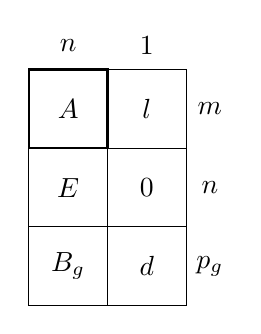
\begin{tikzpicture}
  \draw (0,0)--(2,0)--(2,3)--(0,3)--(0,0);
  \draw (0,1)--(2,1);
  \draw (0,2)--(2,2);
  \draw (1,0)--(1,3);
  \draw (0,0) -- (2,0) -- (2,2) -- (0,2) -- (0,0);
  \draw[thick] (0,2) rectangle (1,3);
  \draw (0.5,2.5) node{$A$};    \draw (0.5,3.3) node{$n$};
  \draw (1.5,2.5) node{$l$};    \draw (1.5,3.3) node{$1$};
  \draw (0.5,1.5) node{$E$};    \draw (2.3,2.5) node{$m$};
  \draw (1.5,1.5) node{$0$};    \draw (2.3,1.5) node{$n$};
  \draw (0.5,0.5) node{$B_g$};
  \draw (1.5,0.5) node{$d$};    \draw (2.3,0.5) node{$p_g$};
\end{tikzpicture}}}}}
%
\end{align*}
%
se základní submaticí $A$. \orig{17} Aplikujeme-li obecné vzorce
(2.20) (2.21) a (2.22) na tento konkrétní případ, vidíme, že zobecněná
ortogonalizace matice $A_0$ povede k matici

\vspace{-5.5mm}
\begin{align*}
%
\tag{3.18}
%
W_0 &= {
\vcenter{\hbox{
{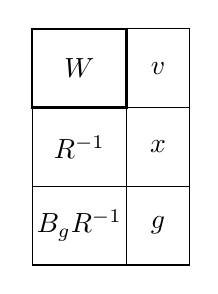
\begin{tikzpicture}[x=1cm,y=1cm]
  \draw (0,0)--(2,0)--(2,3)--(0,3)--(0,0);
  \draw (0,1)--(2,1);
  \draw (0,2)--(2,2);
  \draw (1.2,0)--(1.2,3);
  \draw (0,0) -- (2,0) -- (2,2) -- (0,2) -- (0,0);
  \draw[thick] (0,2) rectangle (1.2,3);
  \draw (0.6,2.5) node{$W$};
  \draw (1.6,2.5) node{$v$};
  \draw (0.6,1.5) node{$R^{-1}$};
  \draw (1.6,1.5) node{$x$};
  \draw (0.6,0.5) node{$B_gR^{-1}$};
  \draw (1.6,0.5) node{$g$};
\end{tikzpicture}}}}}
%
\end{align*}
%


\noindent Docházíme tak k tomuto závěru:\\[1ex]
%
\noindent\emph{Podrobíme-li matici (3.17) zobecněné ortogonalizaci, pak v
pravé části odpovídající matice (3.18) přímo dostaneme opravy $v$,
neznámé $x$ a funkční hodnoty $g$. Kterýkoliv váhový koeficient
dostaneme jako skalární součin odpovídejících řádků v levé části
matice} (3.18).%
\footnote{
Jiného postupu užívá \name{E.SCHMID} [31]. Rovnice oprav (3.1)
převádí na podmínkové rovnice se speciálně definovaným
vektorem absolutních členů a řeší je ortogonalizací.
}
%
Přitom v~konkrétní aplikaci mohou některé submatice ve (3.17)
chybět. Lze např. počítat opravy $v$ i fukční hodnoty $g$, aniž by
byly určovány neznámé $x$.

Využitím výsledků (3.18), příp. alternativním uspořádáním matice $A_0$
můžeme najít řadu dalších důležitých objektů.  Jak ukážeme v odst
3.3.2 lze např. určit pseudoinverzní matici k matici $A$ a
transformační matice pro přímý převod absolutních členů na opravy,
neznámé a funkční hodnoty (viz též [16]). Bezprostředně je zřejmé, že
lze rovněž úsporně zpracovávat úlohy s větším počtem vektorů
absolutních členů.


V případě, že váhy pozorovaných hodnot jsou dány diagonální
maticí $P$ s obecnými prvky ($P \ne E$) , budeme řešit náhradní úlohu,
v níž matice $A$  a $l$ budou zastoupeny maticemi
$\dot A = P^\frac{1}{2}A$ a $\dot l = P^\frac{1}{2}l$.
~Zpracovává se tedy matice
%
\begin{align*}
%
\tag{3.19}
%
A_0 &= {
\vcenter{\hbox{%\setlength{\unitlength}{1cm}
\raisebox{0mm}{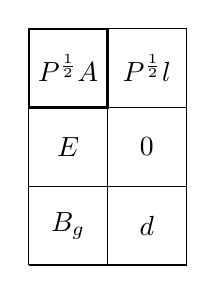
\begin{tikzpicture}[x=1cm,y=1cm]
  \draw (0,0)--(2,0)--(2,3)--(0,3)--(0,0);
  \draw (0,1)--(2,1);
  \draw (0,2)--(2,2);
  \draw (1,0)--(1,2);
  \draw[thick] (0,2) rectangle (1,3);
  \draw (0.5,2.5) node{$P^\frac{1}{2}A$};
  \draw (1.5,2.5) node{$P^\frac{1}{2}l$};
  \draw (0.5,1.5) node{$E$};
  \draw (1.5,1.5) node{$0$};
  \draw (0.5,0.5) node{$B_g$};
  \draw (1.5,0.5) node{$d$};
\end{tikzpicture}}}}}
%
\end{align*}
%

Objekty \orig{18} získané řešením této náhradní úlohy např. podle
vzorců analogických (3.6) až (3.15) označme $\dot O$ na rozdíl od
objektů $O$, které jsou řešením výchozí úlohy. Lze dokázat, že platí
%
{
\newlength{\myl}
\settowidth{\myl}{$Q_{LL}$}
\def\m#1{\makebox[\myl][r]{{$#1$}}}
\begin{align*}
%
\tag{3.20}
%
\begin{array}{lll}
   \m{v} = P^{-\frac{1}{2}}\dot v,  & \m{x} = \dot x,  &   \m{g} = \dot g,\\
   \m{Q_{LL}} = P^{-\frac{1}{2}}\dot Q_{LL}P^{-\frac{1}{2}}, &
   \m{Q_{Lx}} = P^{-\frac{1}{2}}\dot Q_{Lx},   &
   \m{Q_{Lg}} = P^{-\frac{1}{2}}\dot Q_{Lg},\\
   &   \m{Q_{xx}} = \dot Q_{xx}, &  \m{Q_{xg}} = P^{-\frac{1}{2}}\dot Q_{xg},\\
   &   &   \m{Q_{gg}} = \dot Q_{gg}.\\
\end{array}
\end{align*}
}

\noindent\Pozn{}
\name{GRAMOVA-SCHMIDTOVA} ortogonalizace není jedinou metodou pro
přímé řešení rovnic oprav, při které není nutno pracovat se soustavou
normálních rovnic. Jsou známy metody, založené na násobení soustavy
rovnic oprav (3.1) vhodně volenou ortogonální maticí $S$, které rovněž
v podstatě převádějí řešení výchozí soustavy rovnic oprav na mnohem
jednodušší řešení soustavy rovnic s~horní trojúhelníkovou
maticí. Volba matice $S$ i vlastní násobení touto maticí bývají
realizovány různými způsoby. Užívá se např. postupného násobení
elementárními maticemi zrcadlení, tzv. \name{HOUSEHOLDEROVÝCH}
transformací [51].  Naznačený postup má některé přednosti před
\name{GRAMOVOU-CHMIDTOVOU} ortogonalizací - vyžaduje např. menší počet
aritmetických (operací a má i skromnější pamětové nároky. Nevýhoda
metody spočívá v tom, že se nejeví jako příliš vhodná pro vyrovnání
podmínkových pozorování a tedy, že by jen s obtížemi mohla být vzata
za základ univerzálního algoritmu pro řešení všech základních úloh
vyrovnávacího počtu.
